\documentclass[11pt]{article}

\usepackage[a4paper,margin=1in]{geometry}
\usepackage{amsmath}
\usepackage{amssymb}
\usepackage{booktabs}
\usepackage[round,authoryear]{natbib}
\usepackage{hyperref}
\usepackage{tikz}
\usetikzlibrary{arrows.meta,positioning,fit,backgrounds}

\hypersetup{colorlinks=true,linkcolor=black,citecolor=blue,urlcolor=blue}

\newcommand{\E}{\mathbb{E}}
\newcommand{\R}{\mathbb{R}}

\title{\textbf{An EM--Bayesian GVAR:\\ A Unified, Estimable, Real-Time Global Forecasting System}\\[4pt]
\large{(Short paper outline --- with first out-of-sample results)}}
\author{M.\ Farkas}
\date{\today}

\begin{document}
\maketitle

\begin{abstract}
\noindent We integrate four estimation ingredients that the literature has so far deployed
separately---(i) hierarchical Bayesian shrinkage \citep{GiannoneLenzaPrimiceri2019},
(ii) EM data-completion under pervasive, ragged and pandemic-driven missingness,
(iii) endogenous cross-country coupling with an \emph{endogenous} dominant unit, and
(iv) a fiscal stock--flow block---into one deployable global forecaster, the
\emph{EM--Bayesian GVAR}. The object is estimable as a single fixed point and solvable in
real time: per-bloc Bayesian VARs ($p{=}3$) are coupled through trade-weighted ``star''
regressors and US-determined global commons, solved at run time as $x = Mx + d$. Making the
United States endogenous yields global spillover channels a frozen-anchor GVAR cannot
produce. The paper is method-led: the machinery is the engine, global forecasting is the
payoff. In a recursive out-of-sample race over 56 origins (2010Q1--2024Q4) against eight
benchmarks, scored by CRPS and a Model Confidence Set (MCS), the EM--Bayesian GVAR does
\emph{not} win the point race---AR($p$) and a dynamic factor model lead---but it sits
\emph{inside} the MCS on the nominal block (inflation at every horizon, the short rate at
$h\le4$), \emph{decisively beats} the textbook OLS GVAR, and its endogenous-US variant
weakly dominates the frozen one. A US $+100$\,bp conditional projection exposes a
non-trivial RoW$\to$US feedback channel the frozen anchor structurally omits, though its
magnitudes (a multi-period conditional projection, not a causal impulse response) await a
validation pass. The draw-based densities are over-confident, so CRPS---not a parametric
log-score---carries the density conclusions.
\end{abstract}

\section{Introduction}

Global VARs \citep{PesaranSchuermannWeiner2004,DeesDiMauroPesaranSmith2007,ChudikPesaran2016}
deliver cross-country structure but are estimated with fixed weights, balanced panels, and a
weakly-exogenous dominant unit. Bayesian VARs
\citep{Litterman1986,DoanLittermanSims1984,Giannone2015,GiannoneLenzaPrimiceri2019} add shrinkage
and density forecasts; the two have been combined into Bayesian GVARs, but always estimated on the
same balanced panels and with the same weakly-exogenous anchor. Pandemic-era missingness
\citep{LenzaPrimiceri2022,CarrieroClarkMarcellino2015} and ragged real-time vintages
\citep{GiannoneReichlinSmall2008} are then patched by bolt-on cleaning \emph{before} estimation.
Our contribution is not shrinkage or coupling \emph{per se}---both exist---but to fuse data-completion,
shrinkage, and coupling into \emph{one estimable object}: an EM fixed point whose E-step completes the
missing foreign data with the Durbin--Koopman smoother \citep{DurbinKoopman2002,DurbinKoopman2012},
whose M-step re-estimates the coupled Bayesian blocs, and which makes the dominant unit endogenous---all
sharing a common 2025Q4 vintage across $\sim$50 economies (33 GVAR blocs plus 17 euro-area standalones).

\paragraph{Why one estimable object beats bolt-ons.} Treating completion, shrinkage, and coupling
as a single fixed point makes the imputed foreign series, the prior, and the cross-country
weights mutually consistent: the stars a bloc conditions on are the smoothed paths it helps
generate. Contributions:
\begin{itemize}
  \item A \textbf{unified EM--Bayesian GVAR} estimated as one fixed point in the completed
        trade-weighted stars (Algorithm~1), not a pipeline of independent steps.
  \item \textbf{EM completion under pervasive missingness}: COVID macro-masked / financials-observed
        DK imputation, ragged and unbalanced panels, weights renormalized over present partners.
  \item An \textbf{endogenous dominant unit}: the US carries its own RoW stars and a trade-weights
        row, solved via an augmented-state closed form, enabling identified global spillovers.
  \item A \textbf{fiscal stock--flow block} closing debt dynamics by the budget identity with SFA as
        the exact residual, embedded in the same system.
  \item A \textbf{real-time, in-browser deployable} solver ($x{=}Mx{+}d$) with a pre-shipped coupling
        artifact, plus two designed evaluations (forecast horse-race, spillover analysis).
\end{itemize}

\section{The Model}

\paragraph{Per-bloc Bayesian VARs.} For each economy $i$ (a GVAR bloc), stack domestic variables
$y_{i,t}$ and three trade-weighted foreign ``star'' regressors $y^{*}_{i,t}$:
\begin{equation}
  x_{i,t} = \big[\,y_{i,t}^{\prime}\;\; y^{*\prime}_{i,t}\,\big]^{\prime},
  \qquad
  x_{i,t} = c_i + \sum_{\ell=1}^{p} A_{i,\ell}\,x_{i,t-\ell} + u_{i,t},
  \quad p = 3,\;\; u_{i,t}\sim\mathcal{N}(0,\Sigma_i),
  \label{eq:bloc}
\end{equation}
with a hierarchical Minnesota/GLP prior \citep{GiannoneLenzaPrimiceri2019} and Gibbs/Metropolis
sampling of the overall-shrinkage hyperparameter (\texttt{cgl\_bvarV5.m}: $\lambda$ Gamma-prior mode
$0.2$, $\mu$ mode $1$, MH-updated on the full sample).

\paragraph{Trade-weighted stars.} The three stars are foreign-demand, foreign-inflation and
foreign-financial aggregates,
\begin{equation}
  y^{*}_{i,t}\;=\;\sum_{j\neq i} w_{ij,t}\, z_{j,t},
  \qquad
  w_{ij,t} = \frac{\bar w_{ij}\,\mathbf{1}\{j \in \mathcal{P}_{i,t}\}}{\sum_{k\neq i}\bar w_{ik}\,\mathbf{1}\{k\in\mathcal{P}_{i,t}\}},
  \label{eq:stars}
\end{equation}
where $z_{j,t}\in\{\text{ROWDEM},\text{ROWINF},\text{ROWFIN}\}$ and weights are \emph{renormalized over
present partners} $\mathcal{P}_{i,t}$ each quarter (unbalanced panel; the macro stars may use a wider
partner set than ROWFIN, which excludes rate-less or hyperinflation partners).

\paragraph{Solve-time coupling and global commons.} Because each bloc is affine in its pinned
conditioning values (fixed $\widehat A_i,\widehat\Sigma_i \Rightarrow$ DK filter/smoother is affine),
the assembled cross-country system is linear:
\begin{equation}
  x = M x + d
  \qquad\Longrightarrow\qquad
  x = (I - M)^{-1} d ,
  \label{eq:coupling}
\end{equation}
with $x$ the stacked bloc scenario deltas and $M$ the (sparse) star/common transmission map
(\texttt{app/src/lib/compute/gvarSolve.ts}). Four \emph{global commons}---oil, US 10-year yield, US
Baa spread, US equity---are US-determined and pinned 1:1 into every receiving bloc's deviation path.

\paragraph{Endogenous vs.\ weakly-exogenous dominant unit.} In the classical (frozen-anchor) route the
US is weakly exogenous: it has no RoW block, is estimated once, and $M$ is block-lower with the US row
absent. In the endogenous route the US carries its own ROW$^{*}_\text{US}$ stars and a trade-weights
row, so the global channel closes back onto the US and \eqref{eq:coupling} runs on an augmented state.
Spectral radii (from the deployed coupling artifact): $\rho(M)\approx0.59$ (6-bloc pilot),
$0.723$ (24-bloc frozen anchor, $\dim\approx 1380$), $0.924$ (33-bloc endogenous, $\dim\approx 2060$).

\section{Estimation}

The system is estimated as an EM fixed point in the completed stars: the E-step completes foreign data
under missingness (DK smoother), stars are rebuilt from the completed panels, and the M-step
re-estimates each Bayesian bloc; iterate until the stars stop moving.

\begin{quote}
\noindent\textbf{Algorithm 1: EM--Bayesian GVAR fixed-point estimation}\\
(\texttt{pipeline/export\_bvar\_gvar24\_loop.m})
\begin{enumerate}
  \item \textbf{Bootstrap.} Form an initial guess of each foreign star from raw partner data; mask
        the COVID window 2020Q2--Q4 ($3$ quarters), NaN-ing \emph{macro only}
        (domestic macro $+$ ROWDEM $+$ ROWINF); keep all financial columns and ROWFIN observed.
  \item \textbf{E-step (DK completion).} For each bloc, run the Durbin--Koopman smoother inside
        \texttt{cgl\_bvarV5} to impute the macro holes \emph{conditioned on the observed financials},
        giving a completed panel $\widehat X_i = \E[X_i \mid \text{observed}]$.
  \item \textbf{Rebuild stars.} Recompute $y^{*}_{i,t}$ from the completed partner panels via
        \eqref{eq:stars}, renormalizing weights over present partners.
  \item \textbf{M-step (Bayesian estimation).} Re-estimate each bloc \eqref{eq:bloc} by GLP Gibbs on
        $[\,\text{domestic}\mid \text{3 stars}\,]$, updating $(\widehat A_i,\widehat\Sigma_i)$ and the
        hyperparameters.
  \item \textbf{Convergence.} Stop when $\max_i\lVert \Delta y^{*}_i\rVert_\infty < \text{TOL}=0.03$
        (Monte-Carlo floor $\approx 0.13$ excluded), else go to Step~2; cap at $\text{MAXIT}=12$.
\end{enumerate}
\end{quote}

\paragraph{Priors and COVID treatment.} The GLP hierarchical prior shrinks each bloc toward
independent random walks with full-sample-updated shrinkage \citep{GiannoneLenzaPrimiceri2019,Giannone2015}.
COVID is handled as \emph{data-augmentation missingness} (not a volatility rescaling): macro masked,
financials observed, so the smoother fills the pandemic macro holes using the contemporaneous financial
signal---an explicit alternative to outlier down-weighting \citep{LenzaPrimiceri2022,CarrieroClarkMarcellino2015}.

\section{System Features}

\paragraph{Endogenous-US augmented-state closed form.} With the US endogenous, the global commons enter
the state as US-driven deltas, and \eqref{eq:coupling} is solved on an augmented state of dimension
$\dim\approx 2060$. At that size an explicit $(I-M)^{-1}$ is prohibitive in-browser, so the solver is
\emph{inverse-free}: the Neumann fixed point $x \leftarrow d + Mx$ (matvec-only, $O(\dim^2)$/iteration)
converges because $\rho(M)\approx 0.924 < 1$; the frozen-anchor route instead uses
$(I-M)^{-1}$ via Smith doubling. The closed form matches the iterative solve to $<10^{-4}$ and leaves the
legacy 6-bloc path byte-identical.

\paragraph{Fiscal stock--flow block.} Four drivers are estimated---the revenue and primary
expenditure ratios, the effective interest rate EFFI, and the stock--flow adjustment SFA---and
the debt ratio is \emph{derived} by the budget identity
\begin{equation}
  d_t = d_{t-1}\,\frac{1 + i^{\text{eff}}_t/400}{1 + g^{\text{nom}}_t/100} \;-\; \frac{pb_t}{4} \;+\; \frac{\text{sfa}_t}{4},
  \label{eq:debt}
\end{equation}
the standard snowball recursion \citep{Bohn1998,Escolano2010,IMF2013DSA}, with SFA the exact closing
residual (\texttt{app/src/lib/compute/fiscalAccounting.ts}).

\begin{figure}[t]
\centering
\resizebox{\textwidth}{!}{%
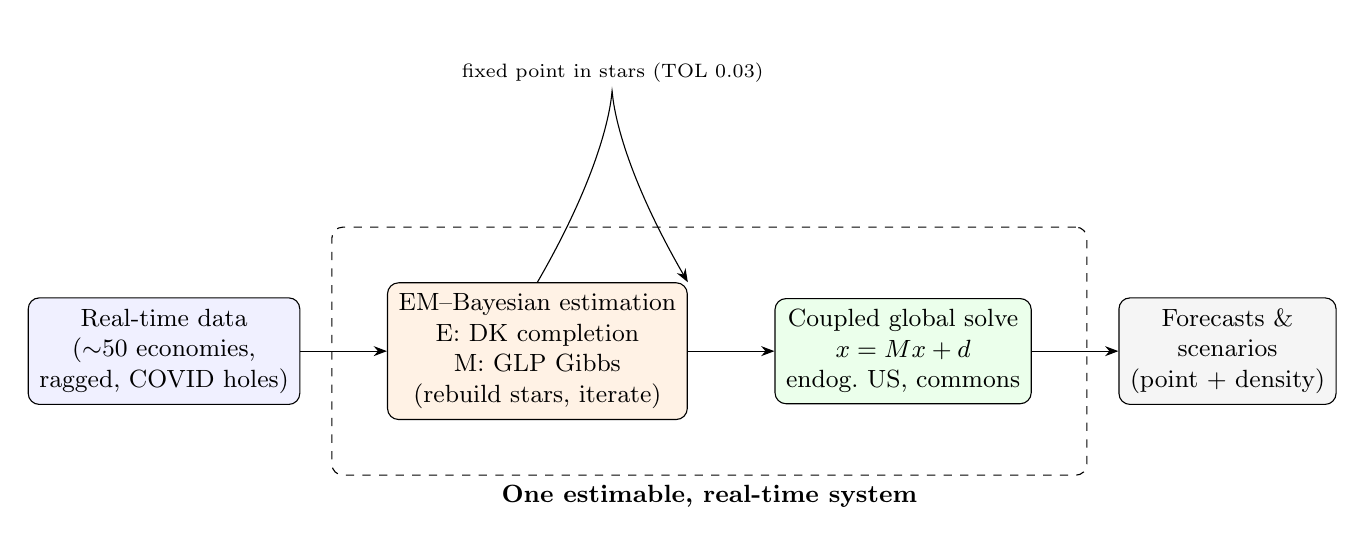
\begin{tikzpicture}[
  >=Stealth, node distance=9mm and 11mm, font=\small,
  box/.style={draw, rounded corners, align=center, minimum height=10mm, inner sep=4pt, fill=white},
  data/.style={box, fill=blue!6},
  est/.style={box, fill=orange!10},
  solve/.style={box, fill=green!8},
  fout/.style={box, fill=gray!8}
]
  \node[data] (data) {Real-time data\\ ($\sim$50 economies,\\ ragged, COVID holes)};
  \node[est, right=of data] (em) {EM--Bayesian estimation\\ E: DK completion\\ M: GLP Gibbs\\ (rebuild stars, iterate)};
  \node[solve, right=of em] (solve) {Coupled global solve\\ $x = Mx + d$\\ endog.\ US, commons};
  \node[fout, right=of solve] (out) {Forecasts \&\\ scenarios\\ (point + density)};

  \draw[->] (data) -- (em);
  \draw[->] (em) -- (solve);
  \draw[->] (solve) -- (out);
  \draw[->] (em.north) to[out=60,in=120,looseness=5] node[above,font=\scriptsize,align=center]{fixed point in stars (TOL $0.03$)} (em.north east);

  \begin{scope}[on background layer]
    \node[draw, dashed, rounded corners, fit=(em)(solve), inner sep=7mm, label=below:{\textbf{One estimable, real-time system}}] {};
  \end{scope}
\end{tikzpicture}}
\caption{System schematic: data $\to$ EM--Bayesian estimation $\to$ coupled global solve $\to$
forecasts/scenarios. The dashed box is the single estimable object.}
\label{fig:system}
\end{figure}

\section{Application 1: An Out-of-Sample Horse-Race}
\label{sec:horserace}

\paragraph{Design.} A recursive/expanding-window pseudo-real-time race on the 2025Q4 vintage. First
origin 2010Q1, last 2024Q4; the four 2020 origins are dropped (an outlier the paper is not about),
leaving 56 nominal origins. \textbf{Trade weights are rebuilt as-of each origin} (rolling
3-year window ending $\le t_0$), the single biggest leakage control; the shipped 2021--2023 weights are
forbidden in the sweep. The headline scope is the six anchor blocs (US, EA, JP, UK, CA, CN) $\times$
\{growth, inflation, short rate\} $\times$ $h\in\{1,2,4,8\}$. Per cell the full-sample benchmarks score
$\sim$55 origins; the GVAR-EM family scores $\sim$51 after the short-sample ($\ge40$q) and stability
trims ($n_{\text{records}}=33{,}912$). Density accuracy is scored by \textbf{CRPS}
\citep{GneitingRaftery2007} as the primary, with a 90\% \textbf{Model Confidence Set}
\citep{HansenLundeNason2011} per (variable, horizon); nesting-correct tests
\citep{GiacominiWhite2006,ClarkWest2007,DieboldMariano1995} (with the Harvey--Leybourne--Newbold
small-sample correction \citep{HarveyLeybourneNewbold1997} and Romano--Wolf step-down
\citep{RomanoWolf2005} for multiplicity) underlie the stars. The benchmark set
(Table~\ref{tab:bench}) ladders from naive to the literature GVAR, with two deliberate
ablations---\texttt{cgvar\_b} (single-pass, no EM re-convergence) isolates the EM star fixed point, and
\texttt{sbvar} (stars stripped) isolates the global coupling.

\begin{table}[t]
\centering
\caption{The nine-model OOS suite. Two proposed variants (D9), six benchmarks, plus a climatology
sibling of the random walk.}
\label{tab:bench}
\begin{tabular}{@{}lll@{}}
\toprule
Model (id) & Cross-country structure & Role / ablation \\
\midrule
Random walk (\texttt{rw}, +\,\texttt{rw\_clim})   & none                       & universal reference \\
AR($p$) (\texttt{arp})                            & none                       & strong univariate dynamic \\
Single-country BVAR (\texttt{sbvar})              & none (per-bloc GLP)        & value of \emph{coupling} \\
Textbook OLS GVAR (\texttt{cgvar\_a})             & fixed weights, exog.\ US, OLS & value of the Bayesian+EM apparatus \\
Single-pass Bayesian GVAR (\texttt{cgvar\_b})     & coupled, $\text{MAXIT}=1$  & value of the \emph{EM star fixed point} \\
Dynamic factor model (\texttt{dfm})               & static factors             & ``is the GVAR structure needed?'' \\
\textbf{EM--Bayesian GVAR, frozen (\texttt{emgvar\_frozen})} & coupled, exog.\ US & legacy anchor \\
\textbf{EM--Bayesian GVAR, endog.\ (\texttt{emgvar\_endo})}  & coupled, endog.\ US & the contribution \\
\bottomrule
\end{tabular}
\end{table}

\paragraph{Result 1: AR($p$) and the DFM lead the point race.} The DFM wins every growth horizon
(CRPS/RW $=0.75/0.84/0.86/0.84$ at $h=1/2/4/8$) and AR($p$) wins inflation and the short rate at the
short--medium horizons (INFL CRPS/RW $=0.63$ at $h{=}1$; RATE CRPS/RW $=0.81$ at $h{=}1$). We state
plainly that the EM--Bayesian GVAR is \emph{not} the point winner.

\paragraph{Result 2: but it is \emph{inside} the Model Confidence Set on the nominal block.}
The 90\% MCS (CRPS loss) places both proposed variants in the \textbf{inflation} set at \emph{all four
horizons}, and \texttt{emgvar\_endo} in the \textbf{short-rate} set at $h=1,2,4$ (out only at $h{=}8$).
\textbf{Growth} is the weak block: the family is out at $h{=}1$ and $h{=}8$, in only at $h=2,4$
(Table~\ref{tab:mcs}). So on the nominal dimension the EM--Bayesian GVAR is statistically
indistinguishable from the best model, despite not minimizing point loss.

\paragraph{Result 3: the endogenous-US design earns its keep, and the textbook GVAR is beaten
decisively.} In the MCS, \texttt{emgvar\_endo} weakly dominates \texttt{emgvar\_frozen}---the decisive
case is the short rate at $h{=}1$, where \texttt{emgvar\_endo} is \emph{in} the set ($p=0.150$) and
\texttt{emgvar\_frozen} is \emph{out} ($p=0.083$). The textbook OLS GVAR (\texttt{cgvar\_a}) is
\emph{out} of many MCS sets and posts the worst relative CRPS in the panel (up to $\approx2.5$ at INFL
$h{=}1$): the Bayesian shrinkage $+$ COVID-as-missing $+$ EM star fixed point is the demonstrable
value-add over the literature GVAR---the cleanest claim the race supports.

\begin{table}[t]
\centering
\caption{90\% Model Confidence Set membership (CRPS loss), six-bloc headline. \checkmark{} $=$ in the
set (indistinguishable from the best). \texttt{emgvar\_frozen} matches \texttt{emgvar\_endo} except
short-rate $h{=}1$, where it is \emph{out}.}
\label{tab:mcs}
\begin{tabular}{@{}lcccc@{}}
\toprule
& \multicolumn{4}{c}{horizon $h$} \\
\cmidrule(l){2-5}
Block ($\to$ \texttt{emgvar\_endo}) & 1 & 2 & 4 & 8 \\
\midrule
Inflation  & \checkmark & \checkmark & \checkmark & \checkmark \\
Short rate & \checkmark & \checkmark & \checkmark & --- \\
Growth     & ---        & \checkmark & \checkmark & --- \\
\bottomrule
\end{tabular}
\end{table}

\paragraph{Honest caveats.} The draw-based densities are \textbf{over-confident}: the GVAR-family 90\%
intervals realize PIT coverage $\approx0.73$--$0.85$ (vs.\ the 0.90 target), worst at $h{=}1$, because
the forecast object propagates only the within-draw shock and $(\beta,\Sigma)$ variation from the
posterior-\emph{mean} completed state and does not integrate the DK-smoother uncertainty of the
COVID-imputed states. The parametric Gaussian \textbf{log-score} is consequently \emph{numerically
broken} on these clouds (magnitudes up to $\sim10^{16}$) and is \textbf{not reported}; \textbf{CRPS and
the MCS}, being calibration-robust, carry every density conclusion.

\section{Application 2: An Endogenous-US Spillover Channel}
\label{sec:spillover}

A US $+100$\,bp \emph{conditional projection}---hold US \texttt{POLRATE} at baseline $+100$\,bp over the
whole 20-quarter horizon---solved under both topologies from the \emph{same} endogenous-staging exports
(the frozen route strips the three $\text{ROW}^{*}_\text{US}$ columns in-memory, so the RoW blocs and
global commons are byte-identical and the gap isolates exactly one channel: US endogeneity). Under the
frozen anchor the US cannot receive any RoW feedback, so its growth/inflation response is the
closed-anchor own-dynamics; under the endogenous solve the global channel closes back onto the US. The
\textbf{gap = endogenous $-$ frozen} is the RoW$\to$US feedback the frozen GVAR structurally cannot
produce (Table~\ref{tab:spillover}): a $+4.2$ (growth) / $+1.3$ (inflation) US gap, with non-trivial,
sign-varying cross-bloc gaps.

\begin{table}[t]
\centering
\caption{US $+100$\,bp conditional projection: peak (max-abs) response by bloc and topology, and the
endogenous$-$frozen gap (scored space; the channel absent under the frozen anchor).}
\label{tab:spillover}
\begin{tabular}{@{}llrrr@{}}
\toprule
Bloc & Var & endo & frozen & gap \\
\midrule
US & growth & $+1.28$ & $-4.37$ & $\mathbf{+4.22}$ \\
   & infl   & $-1.53$ & $-2.82$ & $+1.30$ \\
EA & growth & $+1.04$ & $-0.95$ & $+0.88$ \\
UK & growth & $+2.14$ & $-3.14$ & $+2.94$ \\
JP & growth & $+1.07$ & $+1.62$ & $-1.18$ \\
CN & infl   & $-0.69$ & $+1.19$ & $-1.29$ \\
\bottomrule
\end{tabular}
\end{table}

\paragraph{Honest caveat (not a causal IRF).} This is a \emph{multi-period conditional projection}, not
a structural shock or a generalized impulse response \citep{PesaranShin1998}: the rate path is pinned
over the whole horizon. The qualitative claim---endogenizing the US opens a feedback channel the frozen
anchor cannot represent---is robust; but the magnitudes are large and sign-flipping across blocs, so
they \textbf{await a validation pass} (and ideally a GIRF / Diebold--Yilmaz connectedness build
\citep{DieboldYilmaz2012}, the deferred Tier B) before being headlined causally. The same run doubles as
a solver canary: the closed-form endogenous solve reproduces the iterative fixed point to $<10^{-4}$
across every bloc.

\section{Conclusion}

The EM--Bayesian GVAR shows that Bayesian shrinkage, EM data-completion, endogenous cross-country
coupling with an endogenous dominant unit, and a fiscal stock--flow block can be carried by a
\emph{single} estimable, real-time-solvable system rather than a chain of bolt-ons. The first
out-of-sample evidence is honest: the system does not win the point race, but it sits inside the Model
Confidence Set on the nominal block, decisively beats the textbook OLS GVAR (so the Bayesian$+$EM
apparatus pays for itself), and its endogenous-US design weakly dominates the frozen anchor while opening
a RoW$\to$US spillover channel the latter cannot represent. The open items are scoped and stated:
over-confident densities (widen the bands / integrate the smoother uncertainty) and validating the
conditional-projection spillover magnitudes against a GIRF. The method is the contribution; global
forecasting and the spillover channel are the payoff.

\bibliographystyle{plainnat}
\bibliography{references}

\end{document}
